\chapter{Megvalósítás}\label{ch:MEGVALOSITAS}
\begin{osszefoglal}
	A dolgozat tárgyát képező projekt egy EV3 készletből épített kétkerekű egyensúlyozó robot irányítását valósítja meg hálózaton keresztül, telefonos alkalmazás segítségével. E fejezetben bemutatásra kerülnek a megvalósítás során felmerült problémák, ezek megoldása és a felhasznált technológiák.
\end{osszefoglal}

\section{EV3 programozása}\label{sec:MEGVALOSITAS:lejos}
A LEGO MINDSTORMS kifejlesztett egy programozási környezetet, mely célja, hogy a megépített robotot különböző funkcionalitásokkal lehessen felruházni. E környezet lehetővé teszi a kisebb korosztály számára is a robotok programozását. Különböző grafikus elemekből, úgynevezett blokkokból épül fel a program, amely USB-n keresztül kitelepíthető az EV3 vezérlőegységen futó LEGO MINDSTORMS által fejlesztett firmware-re.
Az előbb említett programozási környezet nem alkalmas komplexebb problémák megoldására. Ezért több firmware-t is kifejlesztettek, melyek magas szintű programozási nyelvek használatát támogatják, ilyen a ROBOTC\footnote{\href {http://www.robotc.net}{http://www.robotc.net}} Carnegie Mellon egyetem fejlesztette ki, amely támogatja a C programozást, illetve megemlíteném még a Debian\footnote{\href{https://www.debian.org/}{https://www.debian.org/}} által kifejlesztett ev3dev-et \footnote{\href{http://www.ev3dev.org/}{http://www.ev3dev.org/}} amely a szkript nyelveket támogatja (Phyton, NodeJS, Ruby) . Esetünkben a leJOS firmware-t használjuk.

A leJOS firmware-t José Solórzano hozta létre 1999 végén és azóta is folyamatosan fejlesztik. Linux alapú, nyílt forráskódú, magába foglalja a JVM-t (Java virtual machine), a neve is rámutat a Java programozhatóságra JOS(Java Operating System). Futtatási környezetet biztosít a Java programozóknak, támogatja az objektum orientált programozást. Mindezek lehetővé teszik a socket alapú kommunikációt, szinkronizálhatóságot, szálak alkalmazását és Java típusok használatát.

Az EV3 vezérlőegységen található négy bemeneti (S1, S2, S3, S4), illetve négy kimeneti (A, B, C, D) port. A bemeneti portok esetén a szenzorok csatlakoztathatjuk, valamint a kimeneti portok esetén a motorokat. A leJOS hozzáférést biztosít ezekhez a portokhoz. Konkrétan meg kell adjuk, hogy milyen porton található a motor, illetve a szenzor. Motorok esetén importálnunk kell \texttt{lejos.hardware.port.MotorPort} csomagot és így elérjük a \texttt{MotorPort} interface-t. Szenzorok esetén is hasonló az eljárás, azzal a különbséggel, hogy ebben az esetben a \texttt{lejos.hardware.port.SensorPort} csomagot kell importáljuk a \texttt{SenzorPort} inteface eléréséhez.

A motorok, illetve a szenzorok példányosításához szükséges megadni a motor vagy szenzor megfelelő portját. A leJOS elrejti a szenzorok implementációját, lehetővé téve a magas szintű absztrakció használatát.

A motorok példányosítása esetén az objektum típusának kiválasztása a motor típusától függ és a mód kiválasztásától. A motor típusát meghatározza a mérete(nagy, illetve közepes motorok). Módok kiválasztása esetén lehetőségünk van szabályzott mód (\ref{motorRegMod} ábrán látható), illetve nem szabályzott mód  (\ref{motorUnregMod} ábrán látható) közti választásra. A motorok nem szabályzott módjának típushierarchiája megtekinthető a \ref{fig:unregMotorHierhachia} ábrán, illetve a szabályzott mód a \ref{fig:regMotorHierhachia} ábrán.

\begin{figure}[!htb]
	\centering
	\minipage{0.5\textwidth}
	\pgfimage[width=0.9\linewidth]{images/unregMotor}
	\captionsetup{justification=centering,margin=1.5cm}
	\caption{Nem szabályzott mód szervomotorok típushierarchia}
	\label{fig:unregMotorHierhachia}
	\endminipage
	\minipage{0.5\textwidth}
	\pgfimage[width=0.9\linewidth]{images/regMotor}
	\captionsetup{margin=1.5cm}
	\caption{Szabályzott mód nagy szervomotorok típushierarchia}
	\label{fig:regMotorHierhachia}
	\endminipage
\end{figure}
 
 A szenzorok esetén az objektum példányosítását követően választjuk ki a lehetséges módok közül a nekünk megfelelőt. Ehhez szükségünk van a \texttt{SensorMode} objektumra, amely a későbbiekben biztosítja e mód metódusait. A szenzoroknak megfelelő objektum esetén a motorokkal ellentétbe, mindegyik származtatja a \texttt{UARTSensor} osztályt, a \ref{fig:gyroHierhachia} ábrán látható.

\begin{figure}[!htb]
	\centering
	\pgfimage[width=0.5\linewidth]{images/gyroSenzor}
	\caption{Giroszkóp szenzor típushierarchia}
	\label{fig:gyroHierhachia}
\end{figure}


A \ref{gyroRateMod} és a \ref{gyroAngleMod} ábrákon látható a leJOS firmware által biztosított két mód, a giroszkóp szenzor használatához. A \texttt{rate} mód a szögsebességet méri, amelyet szög/másodperce -ben kapunk meg. Esetünkben szükségünk van a robot dőlési szögére is, amelyet a \ref{egyensulySubSec} alfejezetben látható \ref{szog} képlet segítségével  kiszámítunk. A \ref{gyroRateMod} ábrán látható az előbb említett mód kiválasztása és ezt követően a mintavételezés, melynek eredménye a \texttt{sample} tömb első eleme lesz. Használható \texttt{angle} módban is, amely \ref{gyroAngleMod} ábrán látható. E mód a szenzor kezdő orientációjához képest mér. A mintavételezés hasonlóan történik, mint az előbb említett módnál, annyi különbséggel, hogy ez esetben szöget mér a kezdő pozíciójához képest. Mindkét mód esetében a \texttt{reset} metódus hívással újra kalibrálhatjuk a szenzort.

\begin{lstlisting}[label=gyroRateMod, caption= Giroszkóp szenzor \texttt{rate} mód használata, language=Java]

float[] sample = new float[1];
EV3GyroSensor gyroSensor =  new EV3GyroSensor(SensorPort.S2);

SampleProvider gyroMode = gyroSensor.getRateMode();

gyro.fetchSample(sample, 0);

\end{lstlisting}

\begin{lstlisting}[label=gyroAngleMod, caption= Giroszkóp szenzor \texttt{angle} mód használata, language=Java]

float[] sample = new float[1];
EV3GyroSensor gyroSensor =  new EV3GyroSensor(SensorPort.S2);

SampleProvider gyroMode = gyroSensor.getAngleMode();

gyro.fetchSample(sample, 0);

\end{lstlisting}

A nagy motorok esetében is két módot biztosít a leJOS firmware, a nem szabályzott (\ref{motorUnregMod} ábra) és a szabályzott (\ref{motorRegMod} ábra) módok.

A motor nem szabályzott mód (\ref{motorUnregMod} ábra) használata esetén az irányítást a \texttt{setPower} metódus hívással valósítjuk meg, amelynek -100 és 100 közötti értéket adhatunk át. Az átadott érték határozza meg, hogy mekkora erőt fejtsen ki a motor, ha az átadott érték pozitív, akkor előre forog, illetve, ha negatív akkor hátra. A \texttt{resetTachoCount}, valamint \texttt{getTachoCount} metódusokkal kezeljük a motorban levő forgásmérő szenzort, melynek számlálójának értékét lekérhetjük vagy lenullázhatjuk. Esetünkben szükséges a pozíció, illetve a sebesség meghatározása, a megvalósításához szükséges az előbb említett metódus által lekérni a két motor fordulat számát, amelyeket átlagoljuk, ezáltal kiszűrjük a szenzor mérésénél keletkezett zajokat. Az így megkapott értéket átalakítjuk szögbe, majd kiszámítjuk a \ref{egyensulySubSec} alfejezetben megjelenő (\ref{sebesseg}) és (\ref{pozicio}) képletek segítségével. A \texttt{stop} metódus hívása esetén a motor blokkolt állapotba kerül.    

A motor szabályzott mód (\ref{motorRegMod} ábra) esetén némely funkcionalitás eltér az előbb említett módhoz képest. Ez esetben a motor sebessége fok/másodperc-ben megadható a \texttt{setSpeed} metódus által. A forgás sebessége függ az akkumulátor töltöttségi szintjétől, a maximális sebessége 740 fok/másodperc. A \texttt{rotate} metódussal adjuk meg, hogy hány fokot forduljon a motor. E metódusnak két változata van. Megadhatjuk csak a fokot, vagy egy logikai értékkel megadható, hogy miután elérte az adott forgási fokot magától megálljon a motor. Ez esetben ha forgás közben meghívódik egy másik metódus, mely parancsot ad a motornak, akkor az előbb kiadott utasítás végrehajtása leáll. A \texttt{waitComplete} metódussal lehetőség van arra, hogy bevárja a forgás befejezését, tehát addig vár, míg végrehajtja a motor az azelőtt kapott utasítást. Az előbb említett mód esetén a pozíciót és a sebességet ki kellet számolni. Ez esetben lehetőség van ezen értékek lekérésére a \texttt{getPosition} és \texttt{getSpeed} metódusok által.

Esetünkben lényeges különbség a két mód között, hogy a szabályzott mód esetén jóval lassabb a motorok reagálási ideje, mint a nem szabályzott mód esetén. E mellett a szabályzott mód használatakor, ha kiadunk egy utasítást, akkor kell figyeljünk, hogy utána ne adjunk olyan más utasítást, amely miatt az előzőt leállítaná.

\begin{lstlisting}[label=motorUnregMod, caption=  A nagy motor \texttt{unregulated} mód használata, language=Java]

EncoderMotor motor = new UnregulatedMotor(MotorPort.A)

motor.resetTachoCount();
motor.setPower(40);

int tacho = motor.getTachoCount();

motor.stop();

\end{lstlisting}

\begin{lstlisting}[label=motorRegMod, caption= A nagy motor \texttt{regulated} mód használata, language=Java]

RegulatedMotor motor = new EV3LargeRegulatedMotor(MotorPort.A);

motor.resetTachoCount();
motor.setSpeed(600);
motor.rotate(720);
motor.waitComplete();
motor.rotate(-460, true);

float position = motor.getPosition();

\end{lstlisting}

Annak érdekében, hogy az EV3 vezérlőegységen futtassuk és könnyedén kitelepítsük a programokat, az Eclipse IDE fejlesztői környezetet használjuk és a leJOS plugin-t, amelyek mindezt megkönnyíti. Abban az esetben, ha nem szeretnénk használni az Eclipse fejlesztői környezetet, lehetőség van az Ant\footnote{\href{http://ant.apache.org/}{http://ant.apache.org/}} build rendszer használatára, amely \texttt{build.xml} konfigurációs állományában megadhatóak a dependenciák. Az Eclipse használata esetén manuálisan át kell másoljuk a dependenciák jar fájljait, az SD kártyára telepített leJOS firmware-t \path{/home/root/lejos/ejre1.7.0_60/lib/ext} mappába, hogy a roboton futó program használni tudja a függőségeit.

Mivel az EV3 vezérlőegységen az alapértelmezett firmware van telepítve, ezért külön SD kártyára fel kell telepíteni a leJOS-t. Legalább 2GB-os SD kártya szükséges de ne legyen 32GB-nál nagyobb és ne SDXC típusú legyen, mert nem ismeri fel az EV3 hardware. Az SD kártyát szükséges formázni FAT32 típusú partícióra. A leJOS számítógépre való telepítése során szükség lesz az 1.7 JDK-ra(Java Development Kit). Az előkészített program segítségével feltelepíthető a leJOS firmware az SD kártyára, ehhez még kell a JRE(Java Runtime Environment) is. Mivel az EV3 ARM9-es processzorral rendelkezik, ezért fontos, hogy a JRE ARM verzióját töltsük le. Sikeres telepítés után az SD kártyát behelyezve az EV3 vezérlőegységbe, elindítható a firmware. Ha az alapértelmezett rendszer indul el, akkor meg kell ismételni az SD kártyára való telepítést. Ezt követően telepítsük az Eclipse plugin-t, majd állítsuk be az EV3\_HOME környezeti változónak a feltelepített leJOS plugin elérési útvonalát (\path{C:\Program Files\leJOS EV3}) és a könyvtárán belüli bin könyvtárat (\path{C:\Program Files\leJOS EV3\bin}) a Path-nek. Ezek a beállítások teszik lehetővé az operációs rendszer számára, hogy futtatás esetén megkapja a szükséges fájlok elérési útvonalát.

\section{Androidos alkalmazás és kommunikáció}\label{sec:MEGVALOSITAS:android}
A projekt része egy telefonos alkalmazás, mely célja, hogy hálózaton keresztül kapcsolódjon a robothoz egy köztes router segítségével és küldje a megfelelő utasításokat, annak érdekében, hogy a felhasználó tudja irányítani a robot mozgását. Az alkalmazást Android stúdióban készítettük és a kommunikációt Java socketen keresztül valósítottuk meg, amit a leJOS, Linux alapú firmware tesz lehetővé.

Az alkalmazás fejlesztésének célja, hogy könnyen, gyorsan csatlakozni tudjon a felhasználó a robothoz és a sikeres csatlakozás után könnyedén irányítani is tudja. A használatának előfeltétele, hogy a robot és az alkalmazást futtató telefon ugyanarra a router-re legyen rácsatlakozva a kapcsolódás és kommunikáció érdekében. 

Az alkalmazást elindítva megadhatjuk a robot IP és PORT címét, amin keresztül csatlakozik. A csatlakozás során ellenőrizzük a bekért adatok helyes formátumát és azt hogy lehetséges vagy sem a kapcsolat. Az alkalmazás kezelését elősegíti egy általunk létrehozott "Remember me" funkcionalitás, mely célja, hogy a legutóbbi IP és PORT címet visszatöltse az alkalmazás élindításakor. E megvalósítása a SharedPreferences API-n keresztül történik, érték és kulcspárok alapján tárolódnak fájlba az adatok. Ezen adatok hozzáférési pontja a SharedPreferences objektum, amely könnyen kezelhető metódusokat biztosít ezek olvasására, illetve írására.

A sikeres kapcsolódást követően egy 2D-s joystick segítségével lehet irányítani a robotot négy irányba. A joystick vizuális megjelenítésére két kört rajzolunk ki. A nagy kör jelöli vizuálisan a határokat a felhasználónak és ezáltal meghatározunk egy konkrét intervallumot az irányításhoz szükséges értékeknek, valamint így kizárjuk annak a lehetőségét, hogy olyan értékeket olvassunk a kisebb kör mozgatásának hatására, amelyek nem megfelelőek. A kisebbik kör segít a felhasználóval tudatni, hogy a nagy kőr peremén belüli rész az általunk értelmezett, illetve figyelembe vett felület a parancsok küldésére. E két kört a telefon képernyőjére canvas segítségével jelenítsük meg (\ref{fig:joystick} ábrán látható), amely felületéhez hozzárendeljük a megfelelő eseményfigyelőt(\texttt{OnTouchListener}). Annak érdekében, hogy a felhasználó ne tudja kimozdítani a nagyobb körön belüli kisebb kört, átalakításokat végzünk koordináták között.

A képernyőt megérintve az eseményfigyelő által, megkapjuk az $x$ és $y$ koordinátákat, ezeket a pontokat átalakítjuk polárkoordinátákba: $$(x,y) \longrightarrow (r,\varphi)$$ $$r=\sqrt{x^2+y^2}$$ $$\varphi=arctg(y,x)$$ Tudva a két kör sugarának különbségét és a polárkoordinátákat, leellenőrizhető, hogy a kis kör a nagy kör sugarán kívül esik vagy sem. Abban az esetben, ha a nagy körön kívül esik a kirajzolási pont, akkor a sugár mentén rajzoljuk ki a kisebb kört a szög függvényében. Ehhez szükséges polárkoordinátából átalakítani euklideszi koordinátába:  $$(r,\varphi) \longrightarrow (x,y)$$ $$x=R\cdot cos(\varphi)$$ $$y=R\cdot sin(\varphi),$$ ahol R a két kör sugarának különbsége.

\begin{figure}[!htb]
	\centering
	\pgfimage[width=0.3\linewidth]{images/joystick}
	\caption{Joystick vizuális megjelenítése}
	\label{fig:joystick}
\end{figure}

Tudva a mozgatás irányát, socketen keresztül a roboton elindított szervernek küldjük a parancsokat, amelyeket továbbit az egyensúlyozásért felelős algoritmusnak. A kommunikációhoz szükséges szervert robot oldalon, az egyensúlyozásért felelős algoritmussal egy időben indítjuk el, külön-külön szálon.

A felhasználó által kapott irányítási parancsok alatt jól definiált értékekről beszélünk. Vagyis, a parancs függvényében más-más értékek előállításával érjük el a megfelelő értékek halmazát, amely szükséges, hogy a szabályzó megfelelően tudja értelmezni a parancsot, tehát a parancsok összetett értékekből állnak. Ezen értékeket egy modell objektumban tároljuk, amely küldésére szükséges a szerializáció használata.

\subsection{Google Protocol Buffers}

A szerializáció, értelmezése szerint, objektumok állapotának adatfolyamba való kiírása illetve kiolvasása. Ezáltal lementhetőek a későbbi felhasználásra és lehetséges távoli eszközökre való küldése az adatoknak. Tehát biztosítja a modell objektumban lementett értékek állapotát.

Az adatok szerializációját illetve titkosítását a Google Protocol Buffers által biztosítjuk, amely lehetővé teszi, hogy megszerkesszük az adatok struktúráját majd egy speciális generátorral létrehozzuk ezen strukturált adatok kezelésére a hozzá tartozó Java osztályt. E létrehozott osztályon keresztül könnyedén kezelhetjük a strukturált adatokat.

A Google Protocol Buffers~\cite{protobuff} használatához létre kell hozzunk egy \texttt{.proto} kiterjesztésű állományt (\ref{gpb} ábra), amelyben definiáljuk az irányításhoz szükséges adataink struktúráját.
A \texttt{.proto} állomány útmutatóként szolgál a speciális kód generátornak, amely legenerálja a struktúrához való hozzáférést biztosító osztályt.
Az állomány első sorában deklaráljuk a csomag(package) nevét, második sorban konkrétan megadjuk a Java csomag hierarchiáját és a harmadik sorban megadjuk az osztály nevet, amellyel rendelkezni fog a legenerált osztály. Abban az esetben, ha nem adunk meg konkrét nevet a \texttt{java\_outer\_classname} mezőben, akkor a \texttt{.proto} fájl nevét fogja megkapni. A további sorokban megadjuk az adattagokat, amelyek rendelkeznek típus névvel. Ez lehet bool, int32, float, double és string. Minden attribútumnak megadunk egy számot, amely egyedi azonosítóként szerepel a bináris kódolás során. Ezeken kívül megadható három típus mező minden attribútumnak, amelyek a következők: \texttt{required, optional, repeated}. A \texttt{required} mezővel beállíthatjuk, hogy az adott attribútum kötelezően értéket kapjon, különbem RuntimeException vagy IOException hibát eredményez.  Az \texttt{optional} mezőt annak az adattagnak állítjuk be, amely nem biztos, hogy értéket kap futási időben, ebben az esetben megadhatunk \texttt{.proto} állományban egy alapértelmezett értéket ennek az adattagnak. A \texttt{repeated} típussal lehetséges annak a jelzése, hogy az adott adattag ismétlődni fog.

\lstinputlisting[label=gpb,caption= Az adatok strukturáját definiáló .proto állomány, language=Java]{progfiles/dataProtos.proto}

Összehasonlítva a Protocol Buffers-t az XML formátummal, az vehető észre, hogy egyszerűbb, kezelhetőbb az adathozzásférést biztosító osztály által és átláthatóbb, mint az XML. A Protocol Buffers használatakor az adathozzáférés metódus hívással megvalósítható, míg az XML esetén \texttt{tag-ek} nevei szerint amelynek meg kell adjuk, hogy hányadik elemére van szükségünk, tehát lényegesen különböző adat hozzáférési idő. Ezen tulajdonságok tudatában választottuk a Google Protocols Buffers-t és, mivel platform független, több lehetőség van a továbbfejleszthetőségre.

\subsection{Robot oldali kommunikáció}

A robot irányításához szükséges telefonos alkalmazással való kapcsolat létrehozása és az általa küldött utasítások értelmezése. Ahogy az előbbiekben is említettem, a kommunikációt Java socketeken keresztül valósítottuk meg.

A robot processzorának teljesítményét tekintve a Google Protocol Buffers a legmegfelelőbb az adatok szerializációjára.

Robot oldalon külön szálon indítjuk a klienst fogadó szervert. Tehát a robot indulásakor függetlenül az egyensúlyozást megvalósító algoritmustól indítjuk a szervert, amely mindaddig él, míg a robot egyensúlyban van.

Klienssel való kapcsolat létrehozása után, mindaddig várja az utasításokat, míg a kapcsolat él. A szerver egyszerre egy klienstől fogad utasításokat, tehát mindaddig, amíg egy adott klienssel kapcsolata van, addig más kliens nem tud kapcsolódni a szerverhez.

A strukturált adatok kinyerése érdekében a Google Protocol Buffers által legenerált hozzáférési osztályt használjuk. Az így megkapott értékeket átadjuk a szabályzó algoritmusnak, amely a hiba számításánál az elvárt értékeknek tekinti a robot dőlési szögét, szögsebességét, pozícióját, sebességét illetően.

\subsection{Automatikus kapcsolódás}

A robot és a telefonos alkalmazás közti kapcsolat automatikus létrehozását, amely felgyorsítja, illetve megkönnyíti a felhasználónak a kapcsolódást a robothoz, a Cling UPnP (\texttt{Universal Plug and Play)})~\cite{upnp} könyvtár által valósítottuk meg.

A Cling UPnP könyvtár az SSDP (\texttt{Simple Service Discovery Protocol})\footnote{\href{https://en.wikipedia.org/wiki/Simple\_Service\_Discovery\_Protocol}{https://en.wikipedia.org/wiki/Simple\_Service\_Discovery\_Protocol}} protokollt használja.

Szerver oldalon annak érdekében, hogy a kliens lássa a hálózaton, úgymond kell "reklámoznia" magát. Ahhoz, hogy a kliens megtalálja az általa keresett szervert, felkell fedezze a hálózaton levő szervereket, tehát "hallgatóznia" kell. Az ehhez szükséges metódusokat tartalmazza az UPnpService objektum. A szerver létre kell hozzon egy \texttt{UPnpService-t}, amelyet futtatnia kell. Függetlenül attól, hogy szerver vagy kliens oldalon vagyunk, erre szükségünk van. Ezt követően hozza kell adjon egy eszközt (\texttt{Device-t}), amelynek meg kell adni egy egyedi azonosítót, típust, amely a verzió, leírást és a szolgáltatást. Ezek mellett egy icon-t is meglehet adni. A szolgáltatás definiálása (\ref{service} ábrán látható) esetén szükséges egy egyedi azonosító és típus megadása, ez esetben a \texttt{@UpnpServiceId} és a \texttt{@UpnpServiceType} meta-annotációkat használhatjuk. A változók, illetve a metódusok esetén is szükséges az annotációk használata. Változók esetében a \texttt{@UpnpStateVariable} használható. Metódusok esetén \texttt{@UpnpAction-el} jelezzük, hogy metódus. Ezen kívül, ha metódus, akkor, ha van bemeneti paramétere a \texttt{@UpnpInputArgument} használható, illetve, ha van visszatérési értéke a \texttt{@UpnpOutputArgument} annotáció használható.

Lehetséges a metaadatok megadása annotációk helyett XML formátumba is. 

\lstinputlisting[label=service,caption= Szolgáltatást definiáló osztály, language=Java]{progfiles/Service.java}

Kliens oldalon létrehozunk egy \texttt{RegistryListener-t}, amely esemény figyelő, értesül, ha valamely szerver állapota módosult a hálózaton. Ha a számunkra megfelelő állapotba került a szerver, akkor leellenőrizhető, hogy rendelkezik-e az általunk keresett szolgáltatás azonosító id-val. Abban az esetben, ha rendelkezik, akkor a szolgáltatásban a meta-annotációkkal felannotált tevékenységeket futtathatjuk az \texttt{ActionInvocation} API segítségével.

A projektünk során a \texttt{Cling UPnp-t} felhasználva a robot létrehoz egy olyan szolgáltatást, amelytől le tudjuk kérni az IP címét. Az alkalmazás azonosítja ezt a szolgáltatást az \texttt{ID-ja} szerint és lekéri az IP címet, amelyet felhasználva létrehozza a kapcsolatot.

\section{Egyensúlyozás problémái}\label{sec:MEGVALOSITAS:pidModositas}

A dolgozat alapjául a Gilyen Hunor által elkészített projektet vettük és ebből indultunk ki, hogy megvalósítsuk a robot négy irányba való irányítását úgy, hogy megtartsa közbe az egyensúlyi állapotát.

Az eredeti projekt struktúrája nem volt előnyös számunkra. E struktúra tartalmazott egy központi osztály, amelyben definiálva volt egy belső osztályt. Ezen osztályon belül került sor az egyensúlyozást megvalósító PID szabályzó implementálása, amely egy szálon volt elindítva, tehát implementálta a \texttt{Runnable} interfészt. A robot szenzoraitól lekérdezett értékek két modell segítségével voltak eltárolva. A program futtatásakor egy \texttt{Thread}\footnote{\href{https://docs.oracle.com/javase/7/docs/api/java/lang/Thread.html}{https://docs.oracle.com/javase/7/docs/api/java/lang/Thread.html}} objektum példányosítódik, amely konstruktorának át lesz adva a \texttt{Runnable} interfészt implementáló szabályzó algoritmus.

A projekt struktúrájának javítása érdekében különválasztottuk a PID szabályzó algoritmust és a giroszkóp szenzor olvasásához szükséges metódusokat. E két osztályt külön szálon indítjuk el. 

A szinkronizálást a \texttt{CyclicBarrier}\footnote{\href{http://tutorials.jenkov.com/java-util-concurrent/cyclicbarrier.html}{http://tutorials.jenkov.com/java-util-concurrent/cyclicbarrier.html}} segítségével valósítottuk meg, amely a Java 7 része. A példányosításakor (\ref{barrier} ábrán látható) megadható, hogy hány szállal szeretnénk dolgozni. Szinkronizálás során a \texttt{await} metódus hívással a szál várakozik mindaddig, míg az összes szál nem hívja meg ezt a metódus. Mikor egy szál meghívja ezt a metódus akkor a \texttt{CyclicBarrier} növeli a számlálóját és mindaddig várakozik a szál, amíg ez a számláló nem éri el a példányosításkor megadott értéket. Valamint létrehoztunk egy központi osztályt, amely feladata a szálak kezelése és a szenzorokhoz, illetve motorokhoz való hozzáférést biztosító objektumok példányosítása. Az eredeti projekt struktúráját átalakítva, a \ref{fig:gyroBoyUML} ábrán látható osztály diagrammal ábrázolt struktúra alakult ki.

\begin{lstlisting}[label=barrier, caption= CyclicBarrier példányosítása , language=Java]

CyclicBarrier barrier = new CyclicBarrier(2);

\end{lstlisting}

Kezdetben az volt az elképzelésünk, hogy különválasszuk a jobb és bal motorokat irányító algoritmust, ezáltal egymástól függetlenné téve őket. Ehhez szükséges volt a szabályzó algoritmus általánosítása, illetve a két motor szinkronizálásának megoldása. Mivel külön szálon fut a giroszkóp kezelése és külön-külön a két motort szabályzó algoritmusa ezért minden iterációban a giroszkóp leolvasását egyszerre kellett végrehajtsák, különben más-más értékekkel dolgoztak, mely egyensúlyvesztést okozott. Ehhez szükséges volt az előbb létrehozott \texttt{CyclicBarrier} konstruktorának átadott értékének növelése eggyel, mivel most már külön-külön kérte le a giroszkóp szenzor értékét a jobb és bal motorokat vezérlő szál. Emellett még egy újabb \texttt{CyclicBarrier} bevezetése volt szükséges, hogy a motorokat is szinkronizáljuk egymáshoz. E módosítást követően a robot rövid időn belül elvesztette az egyensúlyát.

Mivel a robot LCD kijelzője nem megfelelő méretű, hogy tesztelésre alkalmas adatokat jelenítsünk meg futás közben, ezért szükség van a fájlba való kiíratásra és ezt követően az értékek értelmezésére Matlab segítségével. E módszer igen csak időigényes és nehézkes, mivel a túl sok fájlba való írás leterheli a robot processzorát és növelődik egy iterációnak a végrehajtási ideje. Az iterációnként eltelt idő szerint számítsuk a robot sebességét és PID integrált, illetve derivált tagját is. Tehát, ha jelentősen tolódik egy iteráció lefutási ideje, akkor az kritikusan befolyásolja az algoritmus működését.

Az előbb említett tesztelés esetén felmerülő probléma megoldására naplózási keretrendszert alkalmaztunk. Az Slf4J-LOG4J naplózási keretrendszert választottuk, az Slf4J~\cite{slf4j} egy absztrakciós szint, amely a LOG4J~\cite{log4j} naplózási keretrendszer implementációja fölött áll. A konfigurációs XML állományban, szűrök használatával, lehetőségünk van a naplózási szintek  (debug, info, warning, error) elkülönítésére.

\begin{figure}[!htb]
	\begin{center}
		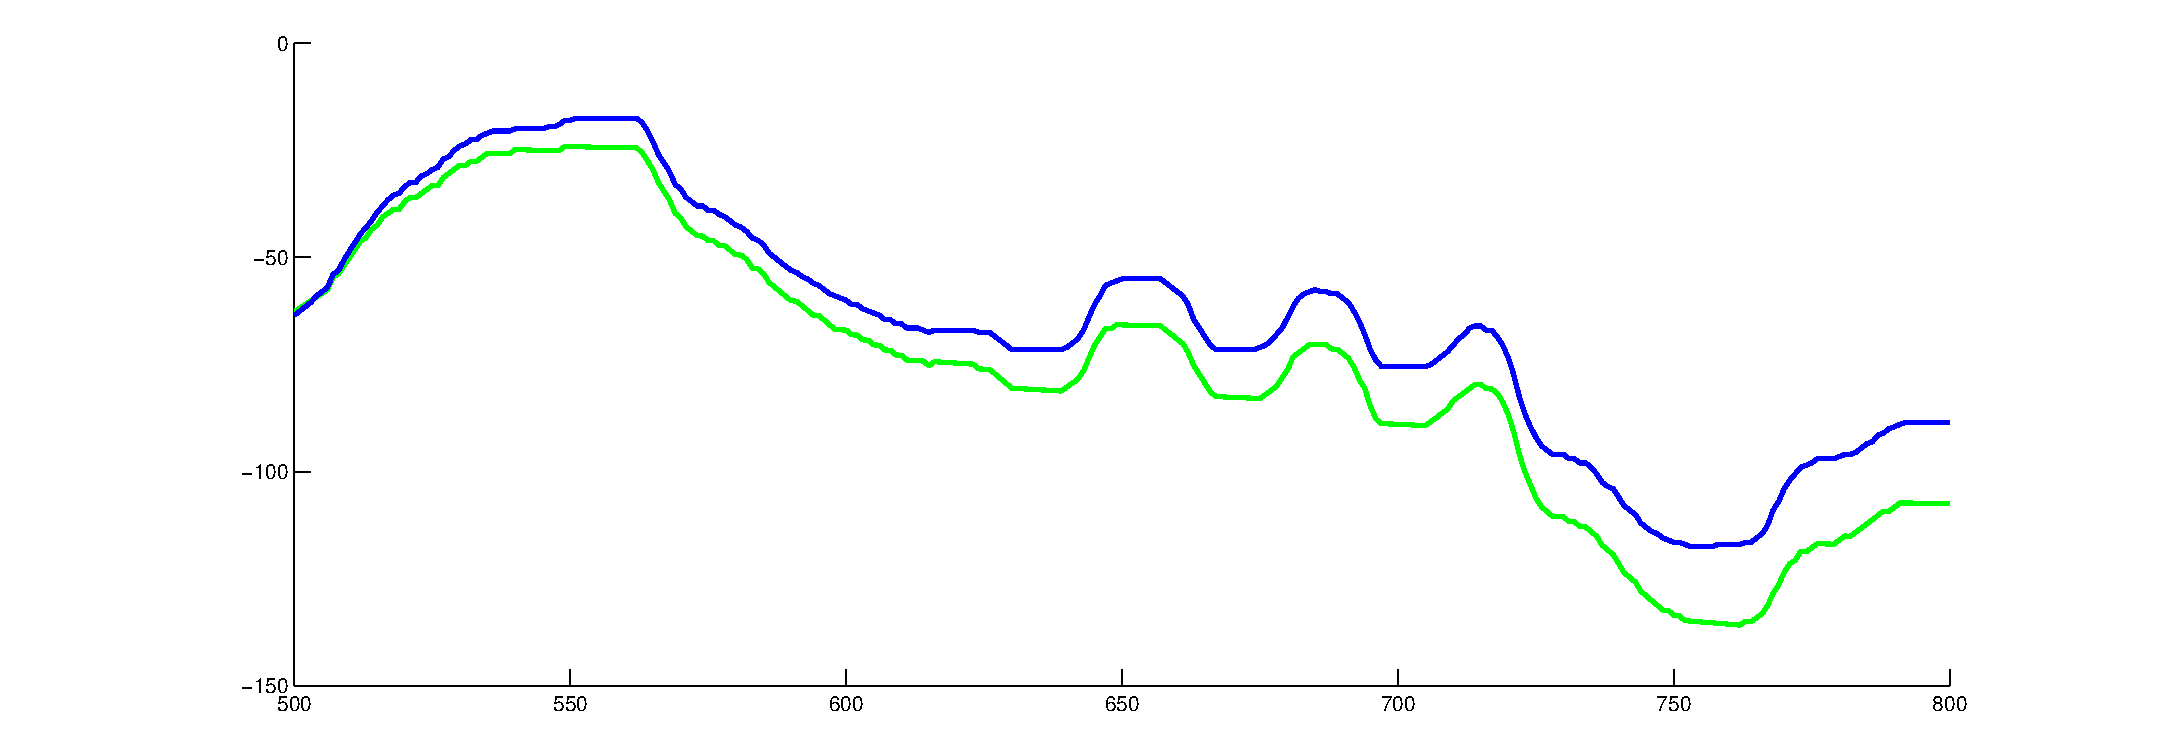
\includegraphics[width=1.0\linewidth]{images/balTacho.eps}
	\end{center}
	\captionsetup{justification=centering,margin=0.5cm}
	\caption[Bal motor fordulatszám összehasonlítása a bal és jobb motor fordulatszám átlagával]
	{Bal motor fordulatszám összehasonlítása a bal és jobb motor fordulatszám átlagával.\\
	Az x tengelyen jelöljük a iterációk számát,	az y tengelyen a fordulatszám értékének mértékét.}
	\label{balTachoFig}
\end{figure}

\begin{figure}[!htb]
	\begin{center}
		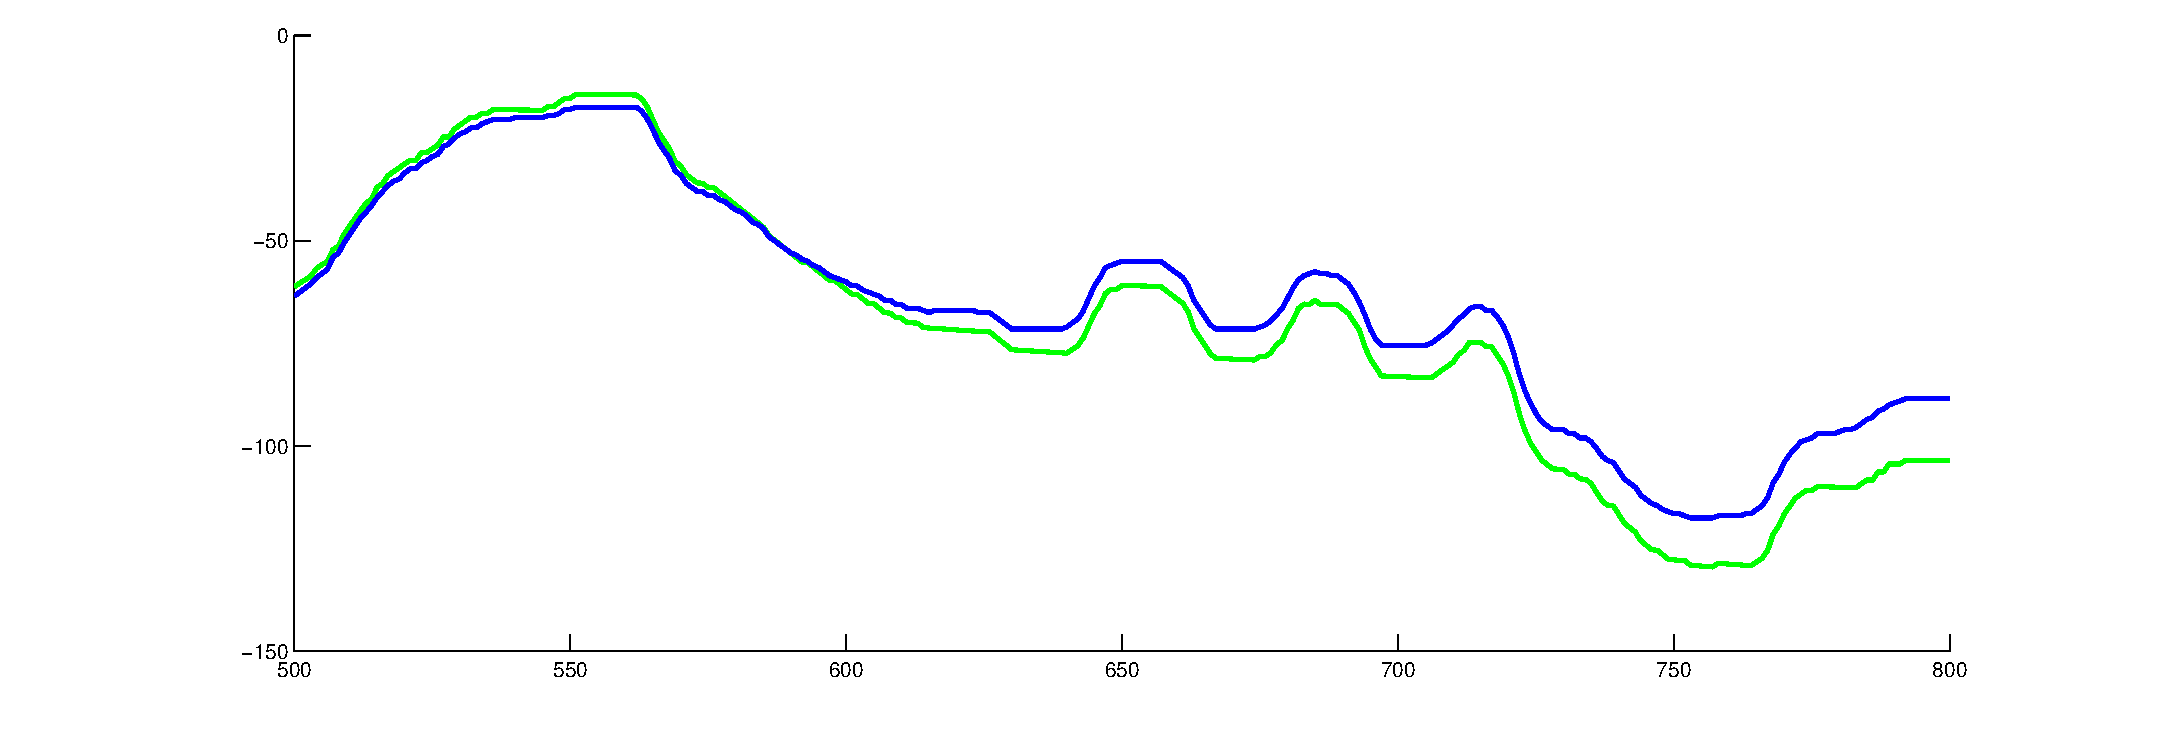
\includegraphics[width=1.0\linewidth]{images/jobbTacho.eps}
	\end{center}
	\captionsetup{justification=centering,margin=0.5cm}
	\caption[Jobb motor fordulatszám összehasonlítása a bal és jobb motor fordulatszám átlagával]
	{Jobb motor fordulatszám összehasonlítása a bal és jobb motor fordulatszám átlagával.\\
	Az x tengelyen jelöljük a iterációk számát,	az y tengelyen a fordulatszám értékének mértékét.}
	\label{jobbTachoFig}
\end{figure}

A szinkronizálás helyességének tesztelése után, a PID szabályzó bemeneti hibáját meghatározó négy komponensnek a kiszámítását teszteltük. Az eredeti projekt szabályzó algoritmusa esetében a robot sebességének és pozíciójának kiszámításakor átlagolva volt a két motor fordulatszáma, annak érdekében, hogy kiszűrje a zajokat. Esetünkben ez módosult és elhagytuk az átlagolást. Ennek eredményeként, amikor egy adott iterációban minimális különbség lépett fel a két motor fordulatszáma között, akkor ez nagymértékben befolyásolta a sebesség és pozíció kiszámítását. Mivel a fordulatszám különbözött, ezért a sebesség és a pozíció is. E különbség iterációnként növekedett. A sebesség és a pozíció a PID bemeneti hibájának a két komponense, ezért a kimeneti érték is különbözött, amely meghatározta a motorokra adott erő nagyságát. Tehát a motorok fordulatmérő szenzorjainak zajos mérései miatt olyan eltérés keletkezett a két motort kezelő szabályzó közt, hogy a robot elvesztette egyensúlyi állapotát.

E probléma megoldására, mivel iterációnként nőtt az eltérés a két párhuzamosan futó szabályzó közt, próbáltuk súlyozni az aktuális és az azelőtti mért fordulatszámot, hogy megközelítsük az átlagolt fordulatszámot. Az így megkapott értékre számoltuk ki a robot sebességét és pozícióját. A legjobb megközelítését, amelyet az átlagolt értékkel hasonlítottunk össze, az látható a \ref{balTachoFig} és a \ref{jobbTachoFig} ábrákon. A kék szín jelöli az adott motor fordulatszámát, illetve a zöld jelöli a motorok átlagolt fordulatszámot. De még ez a közelítés sem volt elegendő, hogy a robot ne veszítse el az egyensúlyát.

\pagebreak
\begin{figure}[h]
	\centering
	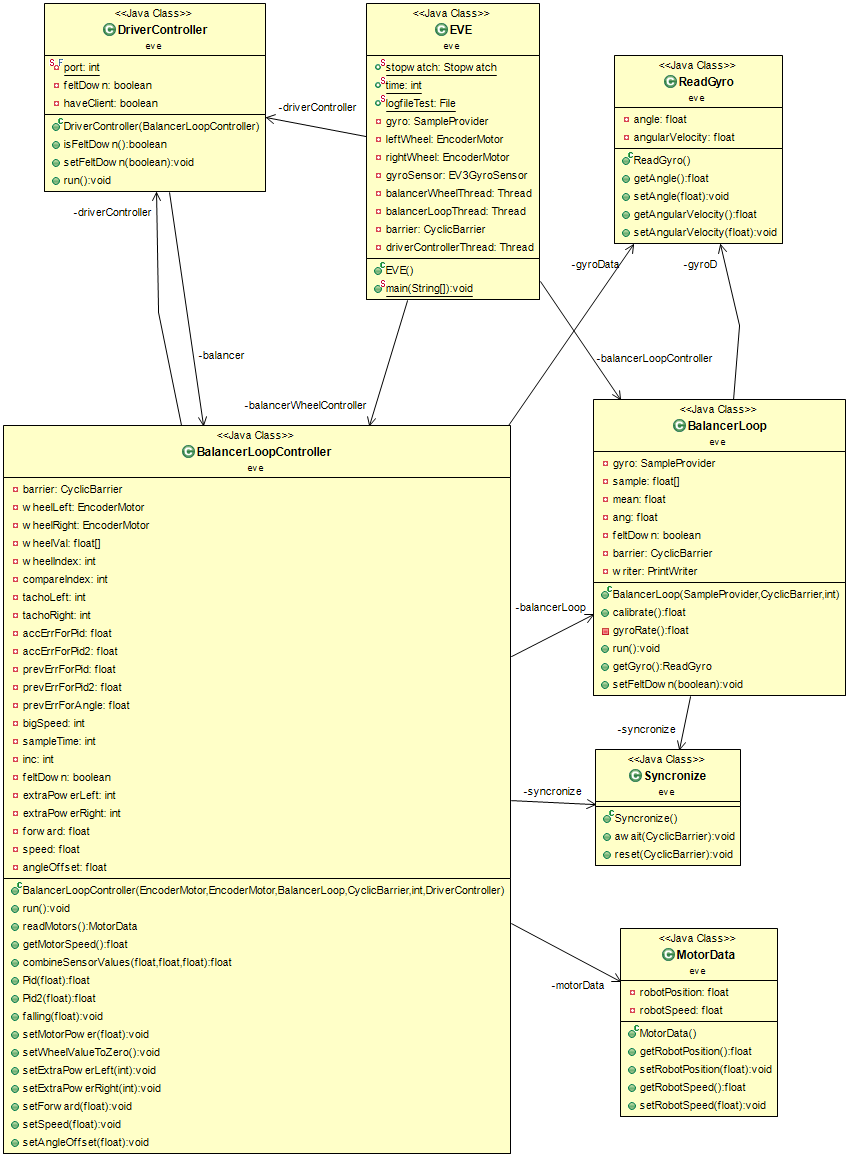
\includegraphics[width=1\textwidth]{images/gyroBoyUML.png}
	\caption{A roboton futó alkalmazás osztály diagramja}
	\label{fig:gyroBoyUML}
\end{figure}
\pagebreak

\subsection{Irányítás megvalósítása és egyensúly megtartása}

Miután sikeresen tudtunk kommunikálni a robottal, nekikezdtünk az irányítás megvalósításának. Rövid időn belül problémába is ütköztünk.

Az első próbálkozásunk során, a motoroknak átadott értéket módosítottuk az irányításnak megfelelően. Jobbra és balra fordulásnál, az iránynak ellentétesen, a megfelelő motornak beállítandó értékét növeltük. Vagyis jobbra fordulásnál növeltük a bal motornak leadott értékét és balra forduláskor a jobb motornak. Ebben az esetben a robot nem a saját tengelye körül fordult, hanem egy hosszabb ívet írt le és eközben a PID szabályzó próbálta kompenzálni a hibát, amit érzékelt. Hiszen hirtelen megnőtt a robot sebessége, hirtelen nagyot változott a pozíciója és megnőtt a dőlési szöge, valamint a szögsebessége. Ennek eredményeként a robot egy-egy pillanatban lelassult, majd felgyorsult. E probléma kiküszöbölésére nem csak a fordulás irányának az ellentettjének megfelelő motor leadott értékét növeltük, hanem ugyan azt az értéket ellentétes előjellel hozzáadtuk a másik motorhoz, vagyis jobbra kanyarodásnál a jobb motor értékéből kivontuk és bal motornak az értékéhez hozzáadtuk. Így a saját tengelye körül fordul. Emellet a szenzorok sem érzékelnek olyan nagy mértékű változást, ami hirtelen befolyásolná a hiba komponenseinek értékét.

Az előre és hátra való irányítás esetén is hasonlóképpen próbálkoztunk, mint a fordulás estében, de ez esetben azonos előjellel módosítottuk a kerekekre leadandó értéket. Ezért kis mértékben elmozdult az iránynak megfelelően, majd a PID szabályzó korrigálta a hibát.

Az első próbálkozásunk után a hiba négy komponensének (szög, szögsebesség, pozíció, robot sebessége) a módosításával próbáltuk elérni, hogy a robot előre vagy hátra fele irányítható legyen. Elképzelésünk szerint próbáltuk a giroszkóp által leolvasott dőlési szög értékét módosítani sikertelenül. Majd a későbbiekben sikerült részleges eredményt elérni. A robot pozíciójának megfelelő változtatásával képesek voltunk a megfelelő irányba elmozdítani a robotot úgy, hogy megtartsa egyensúlyi állapotát. E próbálkozás esetén a pozíció változtatásához bevezettünk egy ellensúlyozást (\texttt{offset}), amely értékét folyamatosan növeltük vagy csökkentettük és hozzáadtuk az aktuális pozícióhoz. Így az egyensúly megtartásához ellensúlyoznia kellett a pozíció értékét. Tehát, ha növeltük az \texttt{offset} értékét a robot hátra ment, ha pedig csökkentettük, akkor előre ment. Ebben az esetben nem mindig volt elég, ha csak egy konstanssal növeltük vagy csökkentettük az \texttt{offset} értékét, így nem volt meg az irányítás alatt egy konstans sebesség. Próbáltuk a szenzor által mért sebesség növelését, de nem oldotta meg a felmerült problémát, csak az előbb említett viselkedést gyorsabban hajtotta végre.

\begin{figure}
	\centering
	\pgfimage[width=1\textwidth]{images/pidSum}
	\caption{PID1 és PID2 szabályzók összekötése}
	\label{pidSum}
\end{figure}


A következő próbálkozásunk esetén ugyancsak a hibát módosítottuk, csak nem az aktuális értékeket, hanem bevezettük az elvárt értéket, ami eddig nulla volt. Emellet rájöttünk, hogy előre és hátra irányítás esetén a hibába szereplő pozíció tagot ki kell vegyük. A pozíció tag esetén a szabályzó arra törekszik, hogy egy helyben maradjon a robot. Tehát, ha előre vagy hátra akarjuk mozdítani a robotot, akkor az irányítás idejére ki kell vegyük ezt a tagot. Ehhez egy újabb PID szabályzó bevezetése volt szükséges, amelynek a bemeneti értéke a pozíció volt, értelemszerűen a másik PID szabályzó hibáját meghatározó komponensek közül kivettük. Tehát, most van egy PID1 és egy PID2 szabályzónk. Irányítás hiányában a két szabályzó kimenetét összegeztük (\ref{pidSum} ára) és ez az érték lett a végleges kimenet, amely a motorokra leadott erőt határozta meg. Irányítás alatt a PID2 szabályzót, amelynek a pozíció megtartásának szabályozása a feladata, nem vettük figyelembe. A PID2 elhagyása, illetve visszavétele kisebb akadály volt, mivel hirtelen csökkent vagy nőtt a szabályzó rendszer kimeneti értéke a derivált tag miatt, hiszen a hiba hirtelen megugrott. E probléma megoldására próbáltuk több iterációra lebontani a különbséget, de ez nem volt elégséges. Megoldása, ha egyensúlyi állapotból irányított állapotba váltunk, akkor az aktuális állapotot vehetjük kiindulási pontnak, mivel a robot egyensúlyban van. Visszaváltás esetén a motorok fordulatszám mérőjét szükséges lenullázni, különben, a PID2 szabályzó túllendülést okoz. Túllendülés alatt azt értem, hogy motoroknak leadandó érték, amely a motor erejét határozza meg. Oly nagy lesz, hogy hirtelen nagyot változik a robot dőlési szöge és elveszti egyensúlyát.
